\documentclass[11pt,a4paper]{article}

% --- Packages ---
\usepackage[utf8]{inputenc}
\usepackage[T1]{fontenc}
\usepackage{geometry}
\geometry{margin=0.8in}
\usepackage{hyperref}
\usepackage{graphicx}
\usepackage{booktabs}
\usepackage{array}
\usepackage{titlesec}
\usepackage{fancyhdr}
\usepackage{enumitem}
\usepackage{caption}
\usepackage{xcolor}
\usepackage{float}
\usepackage[most]{tcolorbox} % For professional frames

% --- Path Configuration ---
\graphicspath{{diagrams/output/plantuml-output/}}

% --- Colors ---
\definecolor{primary}{HTML}{2E5A88}
\definecolor{secondary}{HTML}{E8F0F8}
\hypersetup{
    colorlinks=true,
    linkcolor=primary,
    filecolor=magenta,      
    urlcolor=primary,
}

% --- Header and Footer ---
\setlength{\headheight}{14.5pt}
\pagestyle{fancy}
\fancyhf{}
\fancyhead[L]{\textbf{EduFlow SRS}}
\fancyhead[R]{\thepage}
\fancyfoot[C]{\footnotesize TAJ-LMS Team \textperiodcentered\ 2026}

% --- Formatting ---
\titleformat{\section}{\normalfont\Large\bfseries\color{primary}}{\thesection}{1em}{}
\titleformat{\subsection}{\normalfont\large\bfseries\color{primary}}{\thesubsection}{1em}{}
\setlist[itemize]{noitemsep, topsep=2pt}

% --- Custom Command for Models ---
\newtcolorbox{modelbox}[1]{
    colback=white,
    colframe=primary!50,
    fonttitle=\bfseries,
    title=#1,
    sharp corners,
    boxrule=0.5pt,
    halign=center,
    valign=center,
    drop shadow
}

% --- Document Information ---
\begin{document}

% --- Professional Header ---
\begin{center}
    {\Huge \textbf{Software Requirements Specification}} \\
    \vspace{0.3cm}
    {\LARGE \textbf{EduFlow: E-Learning System}} \\
    \vspace{0.6cm}
    \textbf{Prepared by:} Omama Elzubaier \textperiodcentered\ Olla Sidig \textperiodcentered\ Hager Mouhamed \textperiodcentered\ Ahmed Moumen \\
    \vspace{0.2cm}
    \textbf{Organization:} Arab Academy for Science, Technology \& Maritime Transport \\
    \textbf{Course Lecture:} Dr/Ahmed Salem \textperiodcentered\ \textbf{Repository:} \href{https://github.com/MoUmen-A/LMS-Core-Architecture}{github.com/MoUmen-A/LMS-Core-Architecture} \\
    \vspace{0.4cm}
    \hrule
\end{center}

\tableofcontents
\newpage

% --- Section 1: Introduction ---
\section{Introduction}

\subsection{Purpose}
The purpose of this document is to define the Software Requirements Specification (SRS) for the \textbf{EduFlow: (Student Management And Resource Tracking) E-Learning System}. This document outlines the functional and non-functional requirements of the system, acting as a comprehensive guide for developers, project managers, and stakeholders. It covers the entire scope of the EduFlow system, including user authentication, subscription, scheduling, and lesson management.

\subsection{Document Conventions}
This document follows the IEEE formatting standard for SRS. Priority levels (High, Medium, Low) are assigned to system features to guide the development phases. Requirements are identified by unique tags (e.g., \texttt{REQ-AUTH-1}).

\subsection{Intended Audience and Reading Suggestions}
This document is intended for:
\begin{itemize}
    \item \textbf{Developers \& QA Testers:} To understand technical implementations and write test cases.
    \item \textbf{Project Managers:} To track feature development and define milestones.
    \item \textbf{Stakeholders \& Business Analysts:} To ensure alignment with business objectives.
\end{itemize}
\textit{Suggestion:} Readers are advised to start with Section 2 to grasp the overall system context before proceeding to detailed technical constraints in Sections 3 and 4.

\subsection{Product Scope}
EduFlow is an advanced E-Learning platform designed to streamline online education by connecting students and teachers. Its primary objectives include automating course subscriptions, scheduling classes, processing secure payments, and providing a robust environment for virtual lessons (including file sharing and session recording). By minimizing administrative overhead, EduFlow allows educators to focus on teaching while providing students with a seamless, intuitive learning experience.

\subsection{References}
\begin{itemize}
    \item \textbf{UML Model Output:} \texttt{docs/diagrams/output/plantuml-output/}
    \item \textbf{System Source:} \href{https://github.com/MoUmen-A/LMS-Core-Architecture}{LMS-Core-Architecture Repository}
\end{itemize}

% --- Section 2: Overall Description ---
\section{Overall Description}

\subsection{Product Perspective}
EduFlow is a new, self-contained E-Learning software product. It replaces fragmented educational tools by centralizing scheduling, video lessons, and payment processing into a single web-based application.

\subsection{Product Functions}
Based on the system's architecture, EduFlow provides the following major functions:
\begin{itemize}
    \item \textbf{Authentication \& Security:} Login, Registration, Password Reset, Email Verification, and Admin Approval.
    \item \textbf{Payment \& Subscription:} Course subscription, time-slot selection, automated bank transactions, and discount applications.
    \item \textbf{Scheduling Management:} Availability checking, setting/updating schedules, and lesson rescheduling.
    \item \textbf{Virtual Classroom:} Live lesson conduction, attendance, problem reporting, and session recordings.
    \item \textbf{Resource Management:} Uploading, validating, replacing, and deleting educational materials (PDFs \& Videos).
\end{itemize}

\subsection{User Classes and Characteristics}
\begin{itemize}
    \item \textbf{Student:} Active learners who browse courses, make payments, attend lessons, and report technical issues. Needs an intuitive and highly accessible UI.
    \item \textbf{Teacher:} Educators who set availability schedules, conduct lessons, and upload course materials. Requires a dashboard for resource and schedule management.
    \item \textbf{Admin:} System administrators responsible for verifying/approving new teacher accounts and resolving platform-level issues.
    \item \textbf{Bank (External Actor):} An automated external system responsible for securely processing financial transactions.
\end{itemize}

\subsection{Operating Environment}
\begin{itemize}
    \item \textbf{Platform:} Web-based (accessible via Chrome, Firefox, Safari, Edge).
    \item \textbf{Client Devices:} Desktops, Laptops, and Mobile Devices (Responsive Design).
    \item \textbf{Server:} Cloud-hosted environment (e.g., AWS, Azure) running a modern web server and relational database (e.g., PostgreSQL/MySQL).
\end{itemize}

\subsection{Design and Implementation Constraints}
\begin{itemize}
    \item \textbf{Payment Security:} Must strictly adhere to PCI-DSS standards for processing transactions.
    \item \textbf{Media Hosting:} Video recordings and large PDFs require an optimized cloud storage solution (e.g., AWS S3).
    \item \textbf{Communication Protocol:} All data must be encrypted using HTTPS/TLS.
\end{itemize}

\subsection{User Documentation}
Interactive walk-throughs for new Teachers and Students, alongside an online FAQ and troubleshooting guide for common scheduling or payment issues.

% --- Section 3: External Interface Requirements ---
\section{External Interface Requirements}

\subsection{User Interfaces}
\begin{itemize}
    \item \textbf{Student Dashboard:} Displays upcoming lessons, subscribed courses, and active assignments.
    \item \textbf{Teacher Dashboard:} Displays calendar for scheduling, file management hub, and lesson launching capabilities.
    \item \textbf{Consistency:} Unified design system with standard navigation and modal confirmations.
\end{itemize}

\subsection{Software \& Hardware Interfaces}
\begin{itemize}
    \item \textbf{Hardware:} Access to client device microphones and webcams for Virtual Classroom.
    \item \textbf{Payment API:} Interfaces with Bank Processor for JSON transaction requests.
    \item \textbf{Storage API:} Cloud Storage for saving/retrieving PDFs and MP4 videos.
\end{itemize}

\subsection{Communications Interfaces}
\begin{itemize}
    \item \textbf{HTTPS:} Port 443 for all web traffic to ensure data privacy.
    \item \textbf{SMTP:} For system alerts, email verifications, and notifications.
    \item \textbf{WebRTC/WebSockets:} For low-latency live video streaming and real-time chat.
\end{itemize}

% --- Section 4: System Features ---
\section{System Features}

\subsection{Authentication and User Management}
\textbf{Priority: High.} The system must securely handle user identity, registration, and role-based access. Admin approval is required for teacher accounts.
\begin{itemize}[label=--]
    \item \texttt{REQ-AUTH-1}: Allow users to register as either a Student or a Teacher.
    \item \texttt{REQ-AUTH-2}: Enforce email verification before initial login.
    \item \texttt{REQ-AUTH-3}: Require Admin approval for Teacher accounts before scheduling.
\end{itemize}

\subsection{Payment and Subscription Management}
\textbf{Priority: High.} Students must be able to choose specific slots, apply discounts, and execute payments.
\begin{itemize}[label=--]
    \item \texttt{REQ-PAY-1}: Lock selected slots temporarily while payment is processing.
    \item \texttt{REQ-PAY-2}: Apply valid discount codes to total price before transaction.
    \item \texttt{REQ-PAY-3}: Generate a digital receipt upon successful transaction.
\end{itemize}

\subsection{Scheduling System}
\textbf{Priority: High.} Teachers manage availability; Students and Teachers can request rescheduling based on system rules.
\begin{itemize}[label=--]
    \item \texttt{REQ-SCH-1}: Prevent double-booking of any given time slot.
    \item \texttt{REQ-SCH-2}: Auto-notifications to affected parties if a lesson is rescheduled.
\end{itemize}

\subsection{Virtual Classroom and Lessons}
\textbf{Priority: High.} Core environment for learning with video/audio and problem reporting.
\begin{itemize}[label=--]
    \item \texttt{REQ-CLS-1}: Allow Teachers to start, pause, and end a lesson.
    \item \texttt{REQ-CLS-2}: Allow users to report technical problems during an active session.
    \item \texttt{REQ-CLS-3}: Support automatic uploading of lesson recordings post-session.
\end{itemize}

% --- Section 5: Other Requirements & Rules ---
\section{Other Requirements}

\subsection{Performance \& Security}
\begin{itemize}
    \item Web pages load in under 2.5s; Virtual Classroom latency $<$ 500ms.
    \item Passwords hashed via bcrypt; Sessions expire after 24h inactivity.
    \item Bearer token authentication required for all sensitive data endpoints.
\end{itemize}

\subsection{Software Quality \& Business Rules}
\begin{itemize}
    \item \textbf{Availability:} 99.9\% uptime target. \textbf{Usability:} $<$15 min training for teachers.
    \item \texttt{BR-1}: Payment verified before attending lessons.
    \item \texttt{BR-2}: Admin approval required before teaching.
    \item \texttt{BR-3}: 24-hour notice mandatory for rescheduling.
\end{itemize}

% --- Section 6: Analysis Models (Visualizations) ---
\section{Visual Architecture Models}
\label{sec:models}

\begin{figure}[H]
    \centering
    \begin{minipage}{0.48\textwidth}
        \begin{modelbox}{Use Case Diagram}
            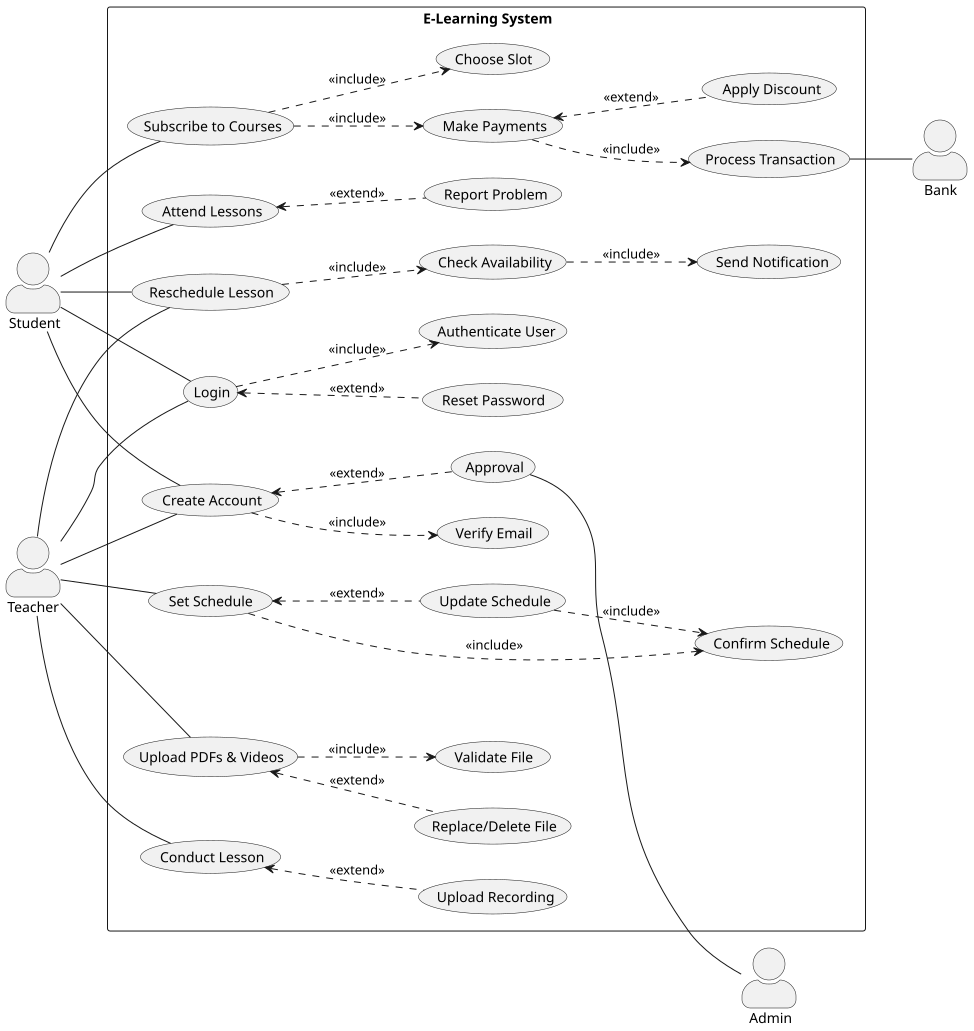
\includegraphics[width=0.9\textwidth]{useCase.png}
        \end{modelbox}
    \end{minipage}
    \hfill
    \begin{minipage}{0.48\textwidth}
        \begin{modelbox}{Class Structure}
            \includegraphics[width=0.9\textwidth]{classDigram.png}
        \end{modelbox}
    \end{minipage}
\end{figure}

\begin{figure}[H]
    \centering
    \begin{minipage}{0.48\textwidth}
        \begin{modelbox}{Payment Process}
            \includegraphics[width=0.9\textwidth]{makePayment.png}
        \end{modelbox}
    \end{minipage}
    \hfill
    \begin{minipage}{0.48\textwidth}
        \begin{modelbox}{Conducting Lesson}
            \includegraphics[width=0.9\textwidth]{conduct-lession.png}
        \end{modelbox}
    \end{minipage}
\end{figure}

\begin{figure}[H]
    \centering
    \begin{minipage}{0.48\textwidth}
        \begin{modelbox}{Student Activity Flow}
            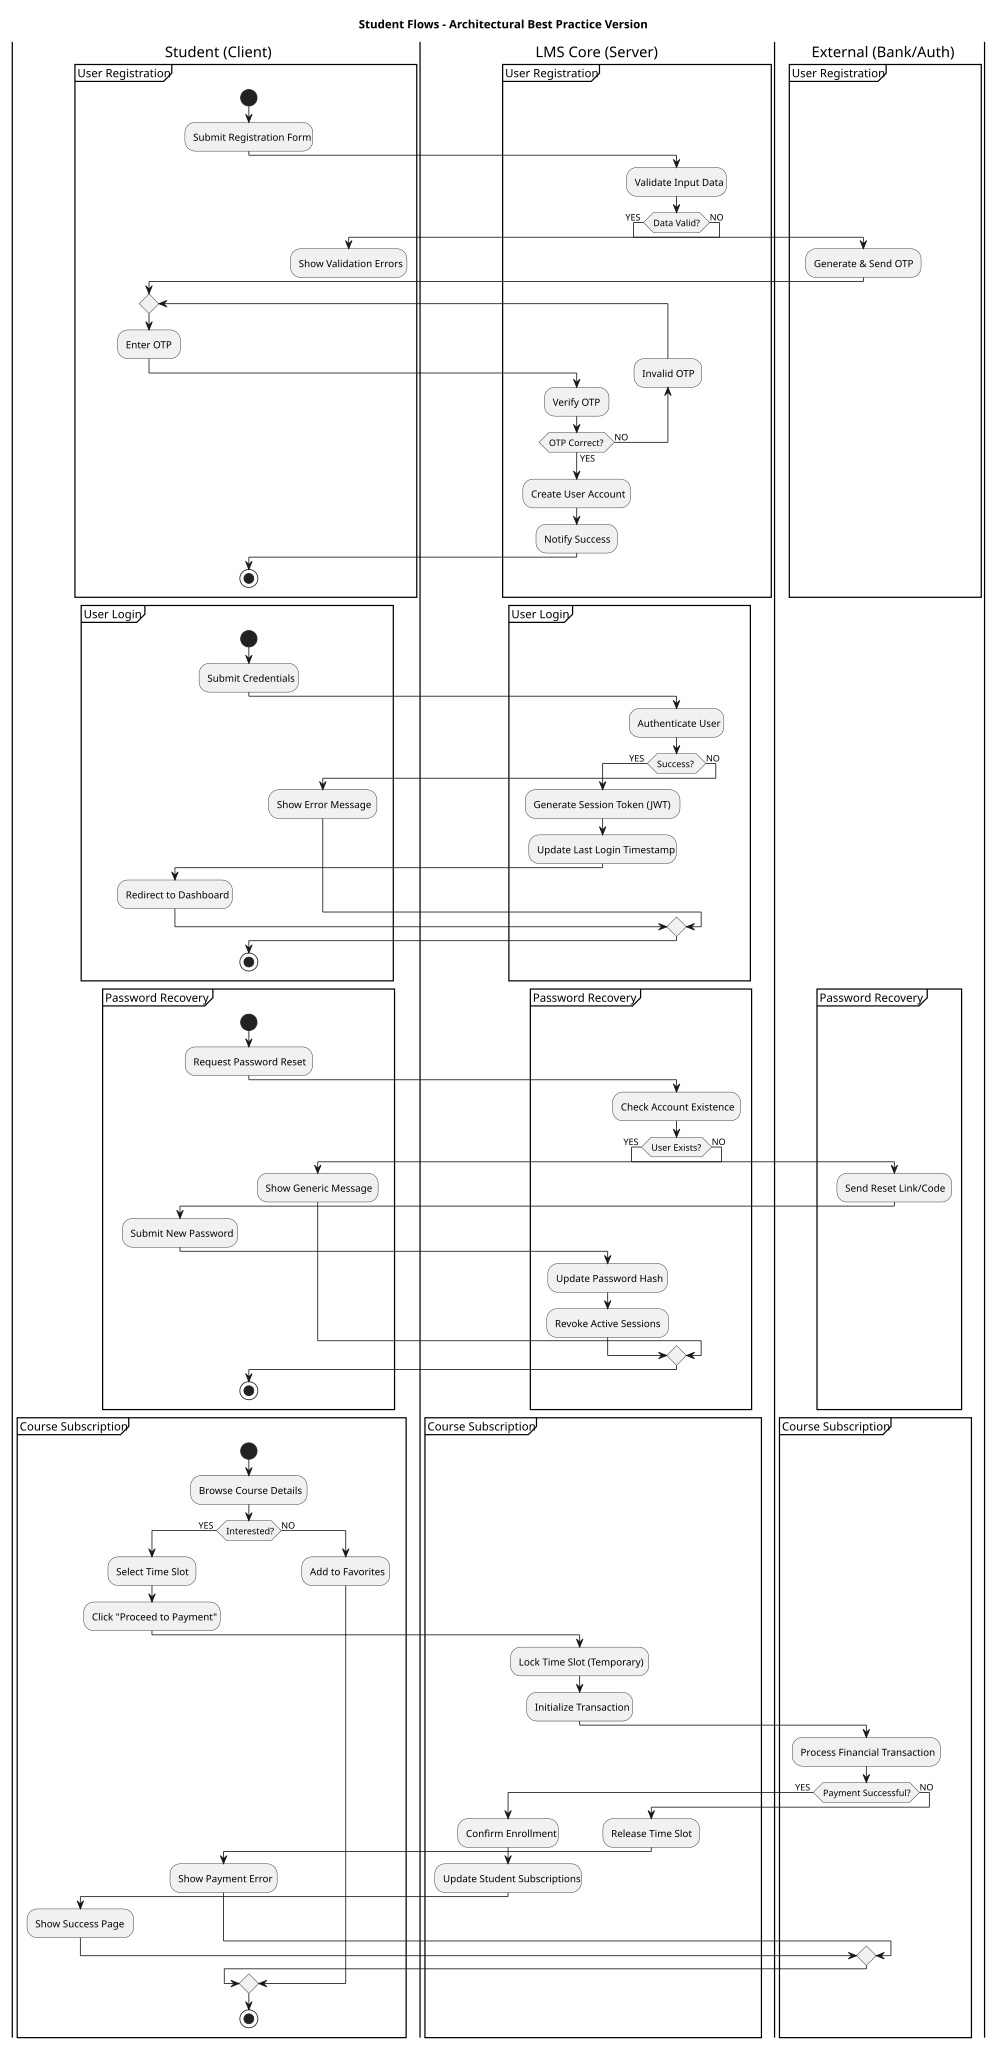
\includegraphics[width=0.9\textwidth]{student_activity_v2_Logicalarchitectural.pdf}
        \end{modelbox}
    \end{minipage}
    \hfill
    \begin{minipage}{0.48\textwidth}
        \begin{modelbox}{Security Misuse Case}
            \includegraphics[width=0.9\textwidth]{misuseCase.png}
        \end{modelbox}
    \end{minipage}
\end{figure}

\section{Appendix}
\textbf{Glossary:} EduFlow (Tracking System), PCI-DSS (Security Standard), WebRTC (Real-time). \\
\textbf{TBD:} Payment provider choice, max file sizes, rescheduling penalties.

\end{document}
